\documentclass[journal,12pt,onecolumn]{IEEEtran}

%--- PREAMBLE ---
% Workaround for conflict between amsmath and txfonts
\let\negmedspace\undefined
\let\negthickspace\undefined

% --- PACKAGES ---
\usepackage[utf8]{inputenc} % Modern input encoding
\usepackage[T1]{fontenc}    % Font encoding for better output
\usepackage{cite}
\usepackage{amsmath,amssymb,amsfonts,amsthm}
\usepackage{algorithmic}
\usepackage{graphicx}
\graphicspath{{./figs/}}
\usepackage{textcomp}
\usepackage{xcolor}
\usepackage{txfonts}
\usepackage{listings}
\usepackage{enumitem}
\usepackage{mathtools}
\usepackage{gensymb}
\usepackage{comment}
\usepackage{caption}
\usepackage{tkz-euclide}
\usepackage{gvv} % Note: This is a non-standard package and requires gvv.sty file
\usepackage{xparse}
\usepackage{array}
\usepackage{longtable}
\usepackage{calc}
\usepackage{multirow}
\usepackage{multicol}
\usepackage{hhline}
\usepackage{ifthen}
\usepackage{lscape}
\usepackage{tabularx}
\usepackage{float}
\usepackage[breaklinks=true]{hyperref} % Should be loaded last

% --- THEOREM DEFINITIONS & CUSTOM COMMANDS ---
\newtheorem{theorem}{Theorem}[section]
\newtheorem{problem}{Problem}
\newtheorem{proposition}{Proposition}[section]
\newtheorem{lemma}{Lemma}[section]
\newtheorem{corollary}[theorem]{Corollary}
\newtheorem{example}{Example}[section]
\newtheorem{definition}[problem]{Definition}
\theoremstyle{remark}

\begin{document}

% --- TITLE & AUTHOR ---
\title{GATE 2020 BT}
\author{EE25BTECH11014 - BHOOMIKA LOKESH}
\maketitle

% Note: The following commands change the numbering of all figures and tables
% to match the main question counter. This can be fragile.
\renewcommand{\thefigure}{\theenumi}
\renewcommand{\thetable}{\theenumi}

\section*{GA - General Aptitude}
\subsection*{Q1-Q5 carry one mark each}

\begin{enumerate}[label=Q\arabic*:]

\item Rajiv Gandhi Khel Ratna Award was conferred   ,Mary Kom, a six-time world champion in boxing, recently in a ceremony      The Rashtrapati Bhawan (the President's official residence) in New Delhi.

\begin{multicols}{2}
\begin{enumerate}

\item with, at
\item on, in
\item on, at 
\item to, at  

\end{enumerate}
\end{multicols}\hfill(GATE BT 2020)

\item Despite a string of poor performances, the chances of K. L. Rahul's selection in the team are .

\begin{multicols}{4}
\begin{enumerate}
\item slim
\item bright
\item obvious
\item uncertain 

\end{enumerate}
\end{multicols}
\hfill(GATE BT 2020)

\item Select the word that fits the analogy: \\
Cover : Uncover :: Associate : 

\begin{multicols}{4}
\begin{enumerate}

\item Unassociate
\item Inassociate
\item Misassociate
\item Dissociate 

\end{enumerate}
\end{multicols}\hfill(GATE BT 2020)

\item Hit by floods, the kharif (summer sown) crops in various parts of the country have been affected. Officials believe that the loss in production of the kharif crops can be recovered in the output of the rabi (winter sown) crops so that the country can achieve its food-grain production target of 291 million tons in the crop year 2019-20 (July-June). They are hopeful that good rains in July-August will help the soil retain moisture for a longer period, helping winter sown crops such as wheat and pulses during the November-February period.\\

Which of the following statements can be inferred from the given passage?
\begin{multicols}{2}
\begin{enumerate}

\item Officials declared that the food-grain production target will be met due to good rains.
\item Officials want the food-grain production target to be met by the November-February period.
\item Officials feel that the food-grain production target cannot be met due to floods.
\item Officials hope that the food-grain production target will be met due to a good rabi produce.

\end{enumerate}
\end{multicols}
\hfill(GATE BT 2020)

\item The difference between the sum of the first 2n natural numbers and the sum of the first n odd natural numbers is .
\begin{multicols}{4}
\begin{enumerate}
\item $n^2 - n$
\item $n^2 + n$
\item $2n^2 - n$
\item $2n^2 + n$
\end{enumerate}
\end{multicols}
\hfill(GATE BT 2020)

\subsection*{Q6-Q10 carry two marks each}

\item Repo rate is the rate at which Reserve Bank of India (RBI) lends to commercial banks, and reverse repo rate is the rate at which RBI borrows money from commercial banks.\\

Which of the following statements can be inferred from the above passage?
\begin{multicols}{2}
\begin{enumerate}
\item Decrease in repo rate will will increase cost of borrowing and decrease lending by commercial banks.
\item Increase in repo rate will decrease cost of borrowing and increase lending by commercial banks.
\item Increase in repo rate will decrease cost of borrowing and decrease lending by commercial banks.
\item Decrease in repo rate will decrease cost of borrowing and increase lending by commercial banks.
\end{enumerate}
\end{multicols}\hfill(GATE BT 2020)

\item  P, Q, R, S, T, U, V, and W are seated around a circular table.
\begin{enumerate}[label=\Roman*.]
    \item S is seated opposite to W.
    \item U is seated at the second place to the right of R.
    \item T is seated at the third place to the left of R.
    \item V is a neighbour of S.
\end{enumerate}
Which of the following must be true?
\begin{multicols}{2}
 \begin{enumerate}

\item\;P is a neighbour of R.
\item\;Q is a neighbour of R.
\item\;P is not seated opposite to Q.
\item\;R is the left neighbour of S.

\end{enumerate}
\end{multicols}
\hfill(GATE BT 2020)

\item The distance between Delhi and Agra is 233 km. A car P started travelling from Delhi to Agra and another car Q started from Agra to Delhi along the same road 1 hour after the car P started. The two cars crossed each other 75 minutes after the car Q started. Both cars were travelling at constant speed. The speed of car P was 10 km/hr more than the speed of car Q. How many kilometers the car had travelled when the cars crossed each other?
\begin{multicols}{4}
\begin{enumerate}
\item\;$66.6$
\item\;$75.2$
\item\;$88.2$
\item\;$116.5$
\end{enumerate}
\end{multicols}
\hfill(GATE BT 2020)

\item  For a matrix M$=$${[m_{ij}]}$$;i,j$=1,2,3,4,the diagonal elements are all zero and ${m_{ij}}=-$${m_{ij}}$. The minimum number of elements required to fully specify the matrix is.
\begin{multicols}{4}
\begin{enumerate}

\item\;$0$
\item\;$6$
\item\;$12$
\item\;$16$

\end{enumerate} 
\end{multicols}\hfill(GATE BT 2020)\\

\item The profit shares of two companies P and Q are shown in the figure. If the two companies have invested a fixed and equal amount every year, then the ratio of the total revenue of company P to the total revenue of company Q, during 2013-2018 
\begin{figure}[H]
    \centering
    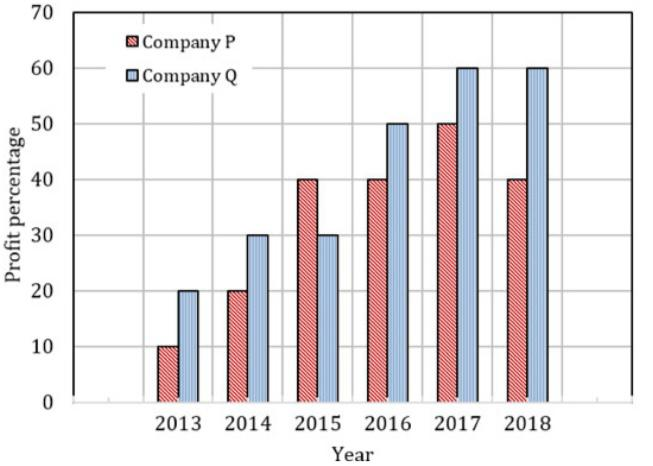
\includegraphics[width=0.6\columnwidth]{figs/graph.jpeg}
    \caption{Profits percentage vs Year}
    \label{fig:graph}
\end{figure}
\begin{multicols}{4}
\begin{enumerate}
\item $15:17$
\item $16:17$
\item $17:15$
\item $17:16$
\end{enumerate}
\end{multicols}
\hfill(GATE BT 2020)
\end{enumerate} 

\section{Q1-Q25 carry one mark each}
\begin{enumerate}[label=Q\arabic*:]
\item Protein P becomes functional upon phosphorylation of a serine residue. Replacing this serine with   will result in phosphomimic mutant of P.
\begin{multicols}{4}
\begin{enumerate}
\item\;alanine
\item\;aspartic acid
\item\;phenylalanine
\item\;lysine
\end{enumerate}
\end{multicols} \hfill(GATE BT 2020)

\item Ras protien is a
\begin{multicols}{2}
\begin{enumerate}
\item\;trimeric GTPase involved in relaying signal from cell surface to nucleus.
\item\;monomeric GTPase involved in relaying signal from cell surface to nucleus.
\item\;trimeric GTPase involved in regulation of cytoskeleton.
\item\;monomeric GTPase involved in regulation of cytoskeleton. 
\end{enumerate}
\end{multicols}
\hfill(GATE BT 2020)

\item Which of the following statements are \textbf{CORRECT}$?$\\
\sbrak{P}Viruses can play a role in causing human cancer\\
\sbrak{Q}A tumor suppressor gene can be turned off without any change in its DNA sequence\\
\sbrak{R} Alteration in miRNA expression levels contributes to the development of cancer
\begin{multicols}{2}
\begin{enumerate}

\item\;P and Q only
\item\;Q and R only
\item\;P and Only
\item\;P,Q and R
\end{enumerate}
\end{multicols}
\hfill(GATE BT 2020)

\item Which class of antibody is first made by developing B cells inside bone marrow?
\begin{multicols}{4}
\begin{enumerate}
\item\;IgG
\item\;IgE
\item\;IgA
\item\;IgM
\end{enumerate}
\end{multicols}
\hfill(GATE BT 2020)

\item Determine the correctness or otherwise of the following Assertion\sbrak{A}Reason\sbrak{R} regarding mammalian cells.\\
Assertion \sbrak{A}:Cells use $Ca^{2+}$, and not $Na^{+}$,for cell-to-cell signaling\\
Reason\sbrak{R}:In the cytosol, concentration of $Na^{+}$ is lower than that of $Ca^{2+}$.
\begin{multicols}{2}
\begin{enumerate}
\item\;Both \sbrak{A} and \sbrak{R} are true and \sbrak{R} is the correct reason for\sbrak{A}
\item\;Both  \sbrak{A} and \sbrak{R} are true and \sbrak{R}is not the correct reason for \sbrak{A}.
\item\ Bhoth  \sbrak{A} and \sbrak{R} are false.
\item\;\sbrak{A} is true but \sbrak{R} is  false.

\end{enumerate}
\end{multicols}
\hfill(GATE BT 2020)

\item Vincristine abd vinblastine, two commercially important secondary metabolites from \textit{Cattaranthus roseus}, are examples of
\begin{multicols}{4}
\begin{enumerate}
\item\;alkaloids.  
\item\;flavonoids.
\item\;terpenoids. 
\item\;steroids.

\end{enumerate} 
\end{multicols}
\hfill(GATE BT 2020)

\item DNA synthesized from an RNA template is called
\begin{multicols}{2}
\begin{enumerate}
\item\;recombined DNA. 
\item\;transcript.
\item\;T-DNA.
\item\;complementary DNA.

\end{enumerate}
\end{multicols}
\hfill(GATE BT 2020)

\item During a positive -negative selection process, transformed animal cells expressing killed in prescence of ganciclovir in the medium.
\begin{multicols}{2}
\begin{enumerate}
\item\;pyruvate kinase
\item\;viral thymidine kinase
\item\;viral serine/threonine kisane  
\item\;viral tyrosine kinase

\end{enumerate}
\end{multicols}\hfill(GATE BT 2020)

\item Two monomeric His-tagged proteins of identical molecular weight are present in a solution. pls of these two proteins are $5.6$ and $6.8$. Which one of the following
techniques can be used to separate them?
\begin{multicols}{2}
\begin{enumerate}

\item\;Denaturing polyacrylamide gel electrophoresis 
\item\;Size-exclusion chromatography
\item\;Ion-exchange chromatography
\item\;Nickel affinity chromatography

\end{enumerate}
\end{multicols}\hfill(GATE BT 2020)

\item A vector derived from which one of the following viruses is used for high-
frequency genomic integration of a transgene in animal cells?
\begin{multicols}{2}
\begin{enumerate}

 \item\;Adeno-associated virus
 \item\;Adenovirus
 \item\;Lentivirus
 \item\;Herpes simplex virus

\end{enumerate} 
 \end{multicols}
\hfill(GATE BT 2020)

\item Which one of the following statements about Agrobacterium Ti plasmid is \textbf{CORRECT}$?$
\begin{multicols}{2}
\begin{enumerate}

\item\;\textit{Vir} genes are located within the T-DNA segment
\item\;Phytohormone biosynthesis genes are located outside the T-DNA segment
\item\;Opine catabolism genes are located within the T-DNA segment
\item\;Opine biosynthesis genes are located within the T-DNA segment

\end{enumerate} 
\end{multicols}
\hfill(GATE BT 2020)

\item Which of the following types of molecules act as biological catalysts?\\
\sbrak{P}Protein\\
\sbrak{Q}RNA\\
\sbrak{R}Phosphoilipid\\
\begin{multicols}{2}
\begin{enumerate}

\item\;P and Q only
\item\;P and R only
\item\;Q and R only
\item\;P, Q and R

\end{enumerate}
\end{multicols}
\hfill(GATE BT 2020)

\item Which one of the following media components is used to maintain pH in mammalian cell culture?
\begin{multicols}{4}
\begin{enumerate}

\item\;$CaCl_2$
\item\;$MgSO_4$
\item\;$NaCl$
\item\;$NaHCO_3$

\end{enumerate} 
\end{multicols}
\hfill(GATE BT 2020)

\item Which of the following are energy transducing membranes?\\
\sbrak{P} Plasma membrane of bacteria\\
\sbrak{Q} Inner membrane of chloroplasts\\
\sbrak{R} Inner membrane of mitochondria
\begin{multicols}{2}
\begin{enumerate}

\item\;P and Q only
\item\;P and R only
\item\;Q and R only
\item\;P, Q and R

\end{enumerate}
\end{multicols}
\hfill(GATE BT 2020)

\item Amino acid sequences of cytochrome c and ribulose 5-phosphate epimerase from 40 organisms were chosen and phylogenetic trees were obtained for each of these two protein families.\\
\\Determine the correctness or otherwise of the following Assertion [a] and the Reason [r].\\Assertion [a]:]: The two trees will not be identical\\
Reason [r]: The nature and frequency of mutations in the two families are
different
\begin{multicols}{2}
\begin{enumerate}

\item\;Both  \sbrak{A} and \sbrak{R}  are true and \sbrak{R}  is the correct reason for \sbrak{A}.
\item\;Both  \sbrak{A} and \sbrak{R}  are true and \sbrak{R} is not the correct reason for \sbrak{A} .
\item\;Both  \sbrak{A}  and \sbrak{R}  are false.
\item\;\sbrak{A}  is true but \sbrak{R}  is  false

\end{enumerate} 
\end{multicols}
\hfill(GATE BT 2020)

\item A microorganism isolated from a salt-rich (salt concentration ~2 M) lake was
found to possess diglycerol tetraethers, with polyisoprenoid alcohol side chains, as the major lipid component of its cell membrane. The isolated organism is
\begin{multicols}{2}
\begin{enumerate}

\item\;a planctomycete
\item\;a cyanobacteria.
\item\;a unicellular amoeba.
\item\;an archaea.
\end{enumerate}
\end{multicols}
\hfill(GATE BT 2020)

\item A function \textit{f} is as follows:\\
\[
f(x) =
\begin{cases}
$15$  & \text{if }x< $ 1$ \\
cx  & \text{if } x \geq $ 0$
\end{cases}
\]

The function \textit{f} is a continuous function when c is equal to .
$\brak{answer\ is\ an \ integer}$.\hfill(GATE BT 2020)

\item Given that \textit{Z }$=$\textit{ X}$^2 +$ \textit{Y}$^2$ , the value of \(\frac{\partial Z}{\partial X}\) for  X$=1 $ and Y$=0 $ is  $\brak{answer\ is\ an \ integer}$.\hfill(GATE BT 2020)


\item The elemental composition of dry biomass of a yeast species is\\
$CH_{1.6}N_{0.2}S_{0.0024}P_{0.017}$. The contribution of carbon to the dry biomass is   \% $\brak{round \ off \ to\ 2 \ decimal\ places}$.\\
Given: atomic weights of H, C, N, O, P and S are$1$, $12$, $14$, $16$, $31$ and $32$, respectively \hfill(GATE BT 2020)

\item Solvents A and B are completely immiscible. Solute S is soluble in both these solvents. 100 g of S was added to a container which has 2 kg each of A and B. The solute is 1.5 times more soluble in solvent A than in solvent B. The mixture was agitated thoroughly and allowed to reach equilibrium. Assuming that the solute has completely dissolved, the amount of solute in solvent A phase is   
\hfill(GATE BT 2020)\\

\item The number of molecules of a nucleotide of molecular weight 300 g/mol present in 10 picomoles is $10^2$ $\brak{round \ off \ to\ 2 \ decimal\ places}$.
\hfill(GATE BT 2020)\\

\item To facilitate mass transfer from a gas to a liquid phase, a gas bubble of radius \textit{r} is introduced into the liquid. The gas bubble then breaks into 8 bubbles of equal radius. Upon this change, the ratio of the interfacial surface area to the gas phase volume for the system changes from $3$/\textit{r} to $3$\textit{n/r}. The value of \textit{n} is  . \hfill(GATE BT 2020)\\

\item The largest eigenvalue of the matrix 
\myvec{4 & 1 \\-2 & 1}
is  . \hfill(GATE BT 2020)\\

\item A normal random variable has mean equal to 0, and standard deviation equal to 3. The probability that on a random draw the value of this random variable is greater than 0 is    $\brak{roundoff\ to\ 2\ decimal\ places}$.\hfill(GATE BT 2020)\\

\item A variable Y is a function of t. Given that Y(t = $0$) =$ 1$ and Y(t =$ 1$) = $2$,$\frac{dY}{dt}$ in the interval \textit{t}=[$0$,$1$]\ can be approximated as .\hfill(GATE BT 2020)
\end{enumerate}

\section{Q26-Q55 carry two marks each.}
\begin{enumerate}[label=Q\arabic*:, start=26, leftmargin=2em]
\item  A block of ice at $0^{\circ}\mathrm{C}$  is supplied heat at a constant rate to convert ice to superheated steam. Which one of the following trajectories correctly represents the trend of the temperature of the system with time? Assume that the specific heat of $H_2O$ is not a function of temperature.
\begin{multicols}{2}
\begin{enumerate}[label=\alph*)]

\item 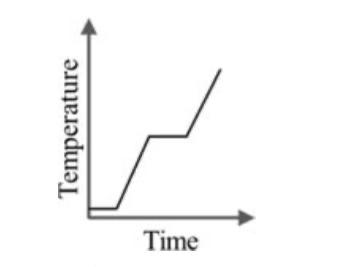
\includegraphics[width=0.4\columnwidth]{figs/fig_1.jpeg}
\item 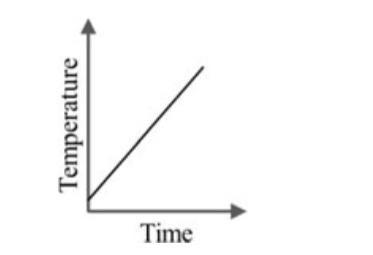
\includegraphics[width=0.4\columnwidth]{figs/fig_2.jpeg}
\item 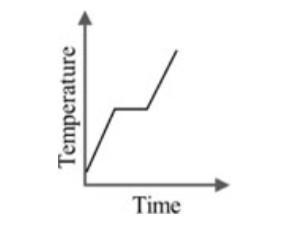
\includegraphics[width=0.4\columnwidth]{figs/fig_3.jpeg} 
\item 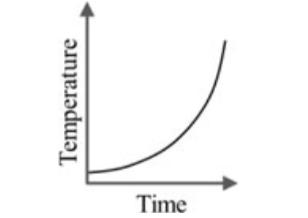
\includegraphics[width=0.4\columnwidth]{figs/fig_4.jpeg}
\end{enumerate}
\end{multicols}
\hfill(GATE BT 2020)


\item The DNA sequence shown below is to be amplified by PCR:\\
5'GCTGAATGATCTGAATTTTCC....TTGGGCGAATAATGAGCCG3'\\
3'GATTCATGAAGCTAAAAAGG.....AACCGTTTATTACTACGCGG5'\\
Which one of the following pair of primers can be used for this amplification?
\begin{enumerate}[label=\alph*)]
\item 5'GGAATTCATGATCTTGATG3' and 5'TTGGGCGAATAATGAGCCG3'
\item 5'GGAATTCATGATCTTGA3' and 5'TTGGGCGAATAATGAGCCG3'
\item 5'GCTGAATGATCTGAATTTT3' and 5'TTGGGCGAATAATGAGCCG3'
\item 5'GGAATTCATGATCTTGATG3' and 5'GGGCGAATAATGAGCCG3'
\end{enumerate}
\hfill(GATE BT 2020)


\item Which of the following statements about immune response are \textbf{CORRECT}?\\
\sbrak{P} T cells are activated by antigen-presenting cells\\
\sbrak{Q} Foreign peptides are not presented to helper T cells by Class II MHC proteins\\
\sbrak{R} Dendritic cells are referred to as professional antigen-presenting cells
\begin{multicols}{2}
\begin{enumerate}[label=\alph*)]
\item P and R only
\item P and Q only
\item Q and R only
\item P, Q and R
\end{enumerate}
\end{multicols}
\hfill(GATE BT 2020)

\item Which of the following statements are \textbf{CORRECT} about eukaryotic cell cycle?\\
\sbrak{P} CDKs can phosphorylate proteins in the absence of cyclins\\
\sbrak{Q} CDKs can be inactivated by phosphorylation\\
\sbrak{R}Degradation of cyclins is required for cell cycle progression\\
\sbrak{S}CDKs are not involved in chromosome condensation

\begin{multicols}{2}
\begin{enumerate}[label=\alph*)]

\item P and R only
\item P and S only
\item P, Q and R only
\item Q and R only

\end{enumerate}
\end{multicols}\hfill(GATE BT 2020)

\item W, X and Y are the intermediates in a biochemical pathway as shown below:\\
\begin{center}
$S{\;\cdots\;}\longrightarrow W\longrightarrow\ X\longrightarrow Y\longrightarrow
Z$\\
\end{center}
Mutants auxotrophic for Z are found in four different complementation groups, namely Z1, Z2, Z3 and Z4. The growth of these mutants on media supplemented with W, X, Y or Z is shown below (Yes: growth observed; No: growth not observed):
\begin{center}
\begin{tabular}{|c|c|c|c|c|}
\hline
\textbf{Mutants} & \multicolumn{4}{c|}{\textbf{Media supplemented with}} \\
\hline
 & W & X & Y & Z \\
\hline
Z1 & No & No & Yes & Yes \\
\hline
Z2 & No & Yes & Yes & Yes \\
\hline
Z3 & No & Yes & No & Yes \\
\hline
Z4 & Yes & Yes & Yes & Yes \\
\hline
\end{tabular}
\end{center}
What is the order of the four complementation groups in terms of the step they
block?\\
\begin{multicols}{2}
\begin{enumerate}[label=\alph*)]
\item $S{\;\cdots\;}\xrightarrow{Z1} W\xrightarrow{Z2} X\xrightarrow{Z3}Y\xrightarrow{Z4}Z$\\

\item $S{\;\cdots\;}\xrightarrow{Z4} W\xrightarrow{Z2} X\xrightarrow{Z1}Y\xrightarrow{Z3}Z$\\

\item $S{\;\cdots\;}\xrightarrow{Z3} W\xrightarrow{Z1} X\xrightarrow{Z2}Y\xrightarrow{Z4}Z$\\

\item $S{\;\cdots\;}\xrightarrow{Z4} W\xrightarrow{Z1} X\xrightarrow{Z2}Y\xrightarrow{Z3}Z$

\end{enumerate} 
\end{multicols}
\hfill(GATE BT 2020)


\item In tomato plant, red \brak{R} is dominant over yellow \brak{r}for fruit color and purple \brak{P} is dominant over green \brak{p} for stem color. Fruit color and stem color assort
independently. The number of progeny plants of different fruit/stem colors obtained from a mating are as follows:\\
Red fruit, purple stem - $145$\\
Red fruit, green stem - $184$\\
Yellow fruit, purple stem-$66$\\
Yellow fruit, green stem - $47$\\

What are the genotypes of the parent plants in this mating?
\begin{multicols}{4}
\begin{enumerate}[label=\alph*)]
\item\textit{RrPp x Rrpp}
\item\textit{RrPpx RrPp}
\item\textit{RRPP x rrpp}
\item\textit{RrPP x Rrpp}
\end{enumerate}
\end{multicols}
\hfill(GATE BT 2020)

\item Some of the cytokinins used in plant tissue culture media are given below:\\
\sbrak{P}BAP\\
\sbrak{Q}Zeatin\\
\sbrak{R}Kinetin\\
\sbrak{S}2iP\\
Which of these are synthetic analogs?
\begin{multicols}{2}
\begin{enumerate}[label=\alph*)]
\item P and Q only
\item Q and S only
\item Q and R only
\item P and R only
\end{enumerate} 
\end{multicols}
\hfill(GATE BT 2020)

\item Carl Woese used the gene sequence of which one of the following for phylogenetic taxonomy of prokaryotes?
\begin{multicols}{2}
\begin{enumerate}[label=\alph*)]
\item A ribosomal RNA of large ribosomal subunit 
\item A ribosomal RNA of small ribosomal subunit
\item A ribosomal protein of large ribosomal subunit
\item A ribosomal protein of small ribosomal subunit\\
\end{enumerate}
\end{multicols}
\hfill(GATE BT 2020)\\

\item A list of pathogens (Group I) and a list of anti-microbial agents (Group II) used to
treat their infections are given below. Match the pathogens with the corresponding anti-microbial agents.
\begin{center}
\begin{tabular}{|c|c|}
\hline
{Group I} & {Group II}\\
\hline
\sbrak{P}Influenza A virus & 1. Isoniazid\\
\hline
\sbrak{Q}Fungus & 2. Amantadine\\
\hline
\sbrak{R} Plasmodium & 3. Fluconazole\\
\hline
\sbrak{S}Mycobacterium & 4. Artemisinin\\
\hline
& 5. Iodoquinol\\
\hline
\end{tabular}
\end{center}

\begin{multicols}{2}
\begin{enumerate}[label=\alph*)]
\item P-4, Q-3, R-2, S-5
\item P-5, Q-2, R-4, S-1
\item P-2, Q-3, R-4, S-1
\item P-2, Q-3, R-1, S-5
\end{enumerate} 
\end{multicols}
\hfill(GATE BT 2020)

\item Determine the correctness or otherwise of the following Assertion \sbrak{a} and the Reason \sbrak{r}.\\
Assertion\sbrak{a}: Dam methylase protects E. coli DNA from phage endonucleases\\
Reason \sbrak{r}: \textit{E. coli} Dam methylase methylates the adenosine residue in the sequence "GATC"

\begin{enumerate}[label=\alph*)]
\item\;Both  \sbrak{a}and \sbrak{r}  are true and  \sbrak{r}is the correct reason for  \sbrak{a}.
\item\;Both   \sbrak{a} and  \sbrak{r} are true and  \sbrak{r}is not the correct reason for  \sbrak{a}.
\item\;Both   \sbrak{a} and  \sbrak{r} are false.
\item\; \sbrak{a} is true but  \sbrak{r} is  false.

\end{enumerate}

\hfill(GATE BT 2020)

\item Determine the correctness or otherwise of the following Assertion \sbrak{a} and the Reason \sbrak{r}.\\
Assertion \sbrak{a} Embryonic stem cells are suitable for developing knockout mice\\
Reason \sbrak{r}: Homologous recombination is more frequent in embryonic stem cells than that in somatic cells

\begin{enumerate}[label=\alph*)]
\item\;Both \sbrak{a} and  \sbrak{r} are false.
\item\;Both \sbrak{a}and \sbrak{r}  are true and  \sbrak{r}is the correct reason for  \sbrak{a}.
\item\;Both \sbrak{a} and  \sbrak{r} are true and  \sbrak{r}is not the correct reason for  \sbrak{a}
\item\;\sbrak{a} is true but\sbrak{r} is  false.
\end{enumerate} 

\hfill(GATE BT 2020)


\item The schematic of a plasmid with a gap in one of the strands is shown below:
\begin{figure}[H]
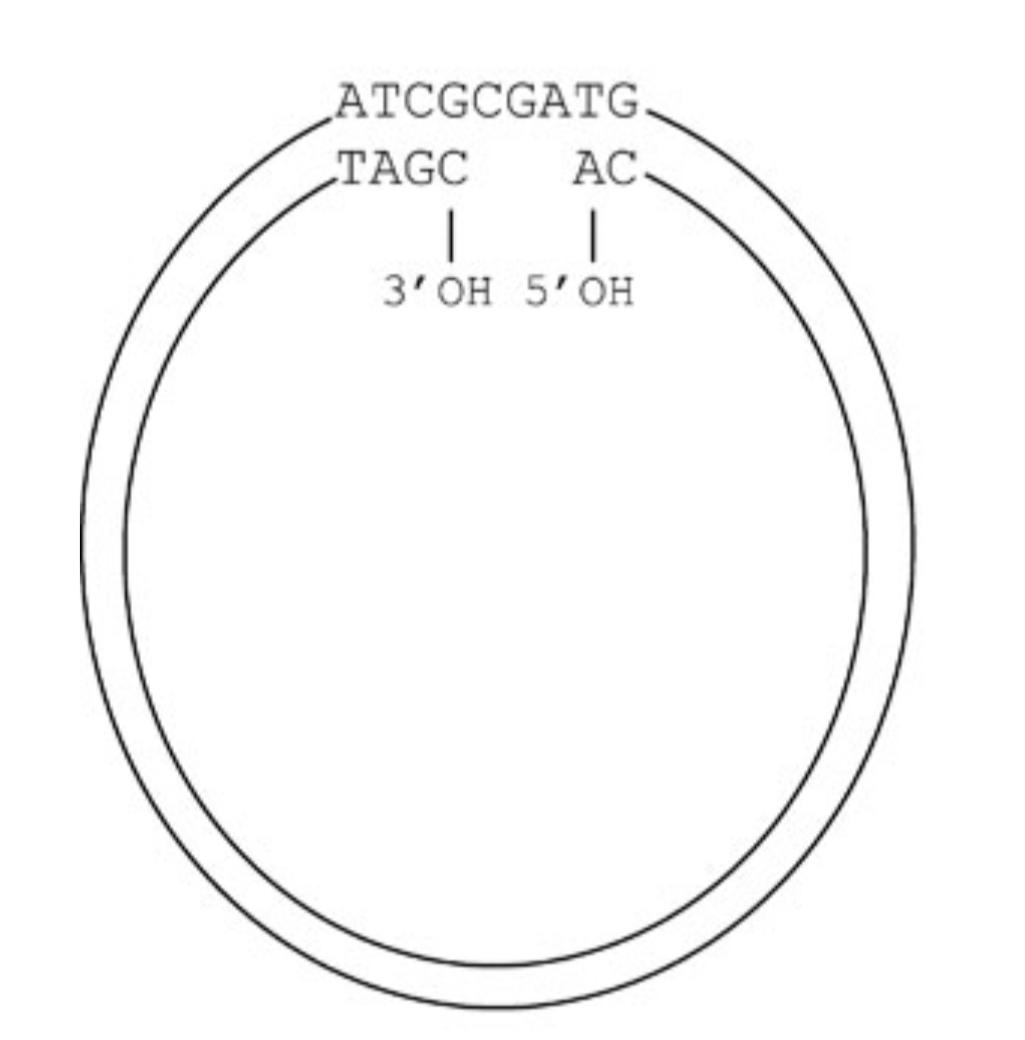
\includegraphics[width=0.3\columnwidth]{figs/figure.jpeg}
\caption{schematic of plasmid}
\label{fig:figure}
\end{figure}

Which of the following enzyme(s) is/are required to fill the gap and generate a covalently closed circular plasmid?\\
\sbrak{P} DNA ligase\\
\sbrak{Q} Alkaline phosphatase\\
\sbrak{R} DNA polymerase\\
\sbrak{S} Polynucleotide kinase\\

\begin{multicols}{2}
\begin{enumerate}[label=\alph*)]

\item\;P only
\item\;P,R and S only
\item\;P and R only
\item\;P,Q and R only 

\end{enumerate} 
\end{multicols}
\hfill(GATE BT 2020)



\item Match sub-cellular organelles listed in Group I with their features listed in Group II:\\
\begin{center}
\begin{tabular}{|c|c|}
\hline
{Group I} & {Group II}\\
\hline
\sbrak{P}Mitochondrion & 1.Single-membrane enclosed\\ 
\hline
\sbrak{Q}Chloroplast & 2.Double-membrane enclosed\\
\hline
\sbrak{R}Nucleus & 3.Maternal inheritance\\
\hline
\sbrak{S}Endoplasmic reticulum & 4.Endodymbiotic origin\\
\hline
\end{tabular}
\end{center}
\begin{multicols}{2}
\begin{enumerate}[label=\alph*)]

\item P-1, Q-4, R-2, S-3
\item P-2, Q-3, R-4, S-1
\item P-3, Q-4, R-2, S-1
\item P-3, Q-1, R-4, S-2

\end{enumerate} 
\end{multicols}
\hfill(GATE BT 2020)

\item Which of the following strategies are used by cells for metabolic regulation?\\
\sbrak{P}Phosphorylation - dephosphorylation\\
\sbrak{Q} Allostery\\
\sbrak{R} Feedback inhibition\\
\begin{multicols}{2}
\begin{enumerate}[label=\alph*)]

\item P and Q only
\item P and R only
\item Q and R only
\item P, Q and R 

\end{enumerate}
\end{multicols}
\hfill(GATE BT 2020)

\item Determine the correctness or otherwise of the following Assertion [a] and the Reason \sbrak{r}.\\
Assertion \sbrak{a}: A zygote and its immediate descendant cells are unspecialized and are called totipotent\\
Reason \sbrak{r}.: Totipotent cells retain the capacity to differentiate into only a few cell types.

\begin{enumerate}[label=\alph*)]

\item\; Both \sbrak{a} and \sbrak{r} are false.
\item\; Both \sbrak{a}and \sbrak{r} are true and \sbrak{r}is the correct reason for \sbrak{a}.
\item\; Both \sbrak{a} and \sbrak{r} are true and \sbrak{r}is not the correct reason for \sbrak{a}
\item\; \sbrak{a} is true but\sbrak{r} is  false.

\end{enumerate} 

\hfill(GATE BT 2020)

\item Which of the following statements about gene therapy are\textbf{CORRECT}?\\
\sbrak{P}Affected individuals, but not their progeny, can be cured through germline gene therapy\\
\sbrak{Q}Affected individuals, as well as their progeny, can be cured through germline gene therapy\\
\sbrak{R}Affected individuals, but not their progeny, can be cured through somatic gene therapy\\\sbrak{S}Affected individuals, as well as their progeny, can be cured through somatic gene therapy

\begin{multicols}{2}
\begin{enumerate}[label=\alph*)]

\item P and R only
\item P and S only
\item Q and R only 
\item Q and S only
\end{enumerate}

\end{multicols}
\hfill(GATE BT 2020)


 \item Determine the correctness or otherwise of the following Assertion \sbrak{a} and the Reason
\sbrak{r}.\\
Assertion \sbrak{a}: A genetically engineered rice that produces beta-carotene in the rice grain is called Golden rice\\
Reason \sbrak{r}: Enabling biosynthesis of provitamin A in the rice endosperm gives a characteristic yellow/orange color \hfill(GATE BT 2020)\\

\begin{enumerate}[label=\alph*)]

\item \;Both \sbrak{a}  and \sbrak{r} are false.
\item\;Both \sbrak{a} and \sbrak{r} are true and \sbrak{r} is the correct reason for \sbrak{a}.
\item\;Both \sbrak{a} and \sbrak{r} are true and \sbrak{r} is not the correct reason for \sbrak{a}.
\item\;Both \sbrak{a} is true but \sbrak{r} is  false.
\end{enumerate}

\hfill(GATE BT 2020)


\item The sequence of a 1 Mb long DNA is random. This DNA has all four bases
occurring in equal proportion. The number of nucleotides, on average, between two successive EcoRI recognition site GAATTC is  . \hfill(GATE BT 2020)\\

\item \textit{E. coli} was grown in $N^{15}$ medium for several generations. Cells were then transferred to $N^{14}$ medium, allowed to grow for 4 generations and DNA was isolated immediately. The proportion of total DNA with intermediate density is is.
$\brak{round \ off \ to \ 2 \ decimal\ places}$. \hfill(GATE BT 2020)\\

\item A batch reactor is inoculated with $1$ g/L biomass. Under these conditions, cells exhibit a lag phase of $30$ min. If the specific growth rate in the log phase is $0.00417$ min', the time taken for the biomass to increase to $ 8 $g/L is min.\\
$\brak{round \ off \ to \ 2 \ decimal\ places}$. \hfill(GATE BT 2020)

\item The system of linear equations\\
\begin{center}
$cx+y=5$\\
$3x+3y=6$\\
\end{center}
has no solution when c is equal to. \hfill(GATE BT 2020)

\item The amino acid sequence of a peptide is Phe-Leu-Ile-Met-Ser-Leu. The number of codons that encode the amino acids present in this peptide is given below:\\
Phe: 2 codons\\
Leu: 6 codons\\
Ile: 3 codons\\
Met: 1 codon\\
Ser: 4 codons\\

The number of unique DNA sequences that can encode this peptide is. \hfill(GATE BT 2020)\\


\item Assume that a cell culture was started with five human fibroblast cells. Two cells did not divide even once whereas the other three cells completed three rounds of cell division. At this stage, the total number of kinetochores in all the cells put together is . \hfill\brak{[GATE 2020-BT]}\\

\item Growth of an organism on glucose in a chemostat is characterized by Monod model with specific growth rate $= 0.45$ $h^{-1}$ and Ks$ = 0.5 $g/L. Biomass from the substrate is generated as Yxs = $0.4$ g/g. The chemostat volume is $0.9 $L and media is fed at $1 $L/h and contains 20 g/L of glucose. At steady state, the concentration of biomass in the chemostat is g/L. \hfill(GATE BT 2020)\\

\item A function \textit{f} is given as:\\

\begin{center}
$\textit{f}\brak{x}= 4X - X^2$
\end{center}
The function \textit{f} is maximized when \textit{X} is equal to. \hfill(GATE BT 2020)\\

\item An infinite series \textit{S} is given as:\\
\textit{S}$=1+ 2/3 + 3/9 + 4/27 + 5/81 +....\brak{to \ infinity}$. 
The value of \textit{S} is\\ $\brak{round \ off \ to \ 2 \ decimal\ places}$ \hfill(GATE BT 2020)\\

\item Protein A and protein B form a covalent complex. Gel filtration chromatography of this complex showed a peak corresponding to $200$ kDa. SDS-PAGE analysis of this complex, with and without beta-mercaptoethanol, showed a single band corresponding to molecular weight $50$ and $25$ kDa, respectively. Given that the molecular weight of protein A is $25$ kDa, the molecular weight of protein B is  kDa. \hfill(GATE BT 2020)\\

\item The concentrations of ATP, ADP and inorganic phosphate in a cell are $2.59, 0.73$ and $2.72$ mM, respectively. Under these conditions, free energy change for the synthesis of ATP at $37^{\circ}\mathrm{C}$ is kJ/mol$\brak{round \ off \ to \ 2 \ decimal\ places}$\\
Given: free energy change for ATP hydrolysis under standard conditions is $-30.5$kJ/mol and R$ = 8.315$ kJ/mol.K \hfill(GATE BT 2020)

\item An algorithm was designed to find globins in protein sequence databases. A database which has 78 globin sequences was searched using this algorithm. The algorithm retrieved 72 sequences of which only 65 were globins. The sensitivity of this algorithm is\%  $\brak{round \ off \ to \ 2 \ decimal\ places}$ \hfill(GATE BT 2020)\\

\item The mitochondrial electron transfer chain oxidizes NADH with oxygen being the terminal electron acceptor. The redox potentials for the two half-reactions are given below:\\

\begin{align*}
\text{NAD}^+ + \text{H}^+ + 2e^- &\rightarrow \text{NADH}, \quad E^\circ = -0.32\, \text{V} \\
\frac{1}{2}\text{O}_2 + 2\text{H}^+ + 2e^- &\rightarrow \text{H}_2\text{O}, \quad E^\circ = 0.816\, \text{V}
\end{align*}

The free energy change associated with the transfer of electrons from NADH to $O_{2}$ is 
\\Given: F = $96500$ C/mol. \hfill(GATE BT 2020)
\end{enumerate}
\end{document}


